\chapter[Planteamiento del problema]{Un problema abierto: por qué la orientación académica sigue siendo artesanal}
\label{ch:problema}

Si los datos son públicos y las técnicas de recuperación de información llevan décadas de madurez, cabe preguntarse por qué la búsqueda de tutor sigue resolviéndose, en la práctica, de forma artesanal.
La respuesta no está en una única barrera insalvable, sino en la \emph{conjunción} de varias dificultades de naturaleza distinta (de ingeniería de datos, lingüísticas, metodológicas y organizativas) que, combinadas, han mantenido el problema sin resolver.
Este capítulo las analiza una a una y concluye destilando los requisitos que cualquier solución realista debe satisfacer.

\section{Información pública, pero no operativa}
\label{sec:problema-datos}

El Portal Científico de la UPM está diseñado para la consulta humana, ficha a ficha.
No ofrece una interfaz programática de acceso a los datos, los identificadores de los investigadores no están publicados como un censo descargable y la información de cada perfil se sirve como HTML semiestructurado cuya organización interna no está documentada ni garantizada en el tiempo.

Las capturas de la Figura~\ref{fig:portal} muestran el aspecto real de un perfil en el portal, la materia prima de la que parte el sistema: una ficha perfectamente legible \emph{de una en una}, pero cuya comparación masiva (decenas o cientos de perfiles) para hallar al tutor idóneo es justamente el esfuerzo manual que el portal no resuelve.

Las dos primeras capturas muestran lo que encuentra el usuario nada más acceder a un perfil.
La Subfigura~\subref{fig:portal-1} recoge las secciones en que se divide la ficha —Presentación, Trayectoria profesional, Bibliometría, Proyectos y transferencia, Docencia, Red, y Resultados y actividad— y corresponde a la primera de ellas, la Presentación.
Todos los perfiles comparten esta estructura: la Presentación reúne las afiliaciones del \gls{pdi}, un breve resumen de su trayectoria (no todos lo tienen y, al parecer, lo genera automáticamente la \gls{upm}) y un gráfico con los temas en los que es experto.
La Subfigura~\subref{fig:portal-2} amplía ese gráfico de temas, con uno de ellos resaltado para ilustrar cómo se presenta en la interfaz.

La Subfigura~\subref{fig:portal-3} muestra la última sección, Resultados y actividad, la más relevante para este trabajo, pues concentra la evidencia que el sistema explota: publicaciones, proyectos y trabajos supervisados.
La sección ofrece varios controles para filtrar esa actividad, pero solo dentro del perfil de un investigador: ayudan a explorar a una persona, no a comparar a muchas.
Se confirma así la barrera de partida: el portal está pensado para la consulta uno a uno, no para una búsqueda a escala sobre todo el \gls{pdi} de la \gls{upm}.

\begin{figure}[htbp]
  \centering
  \begin{subfigure}{0.48\textwidth}
    \centering
    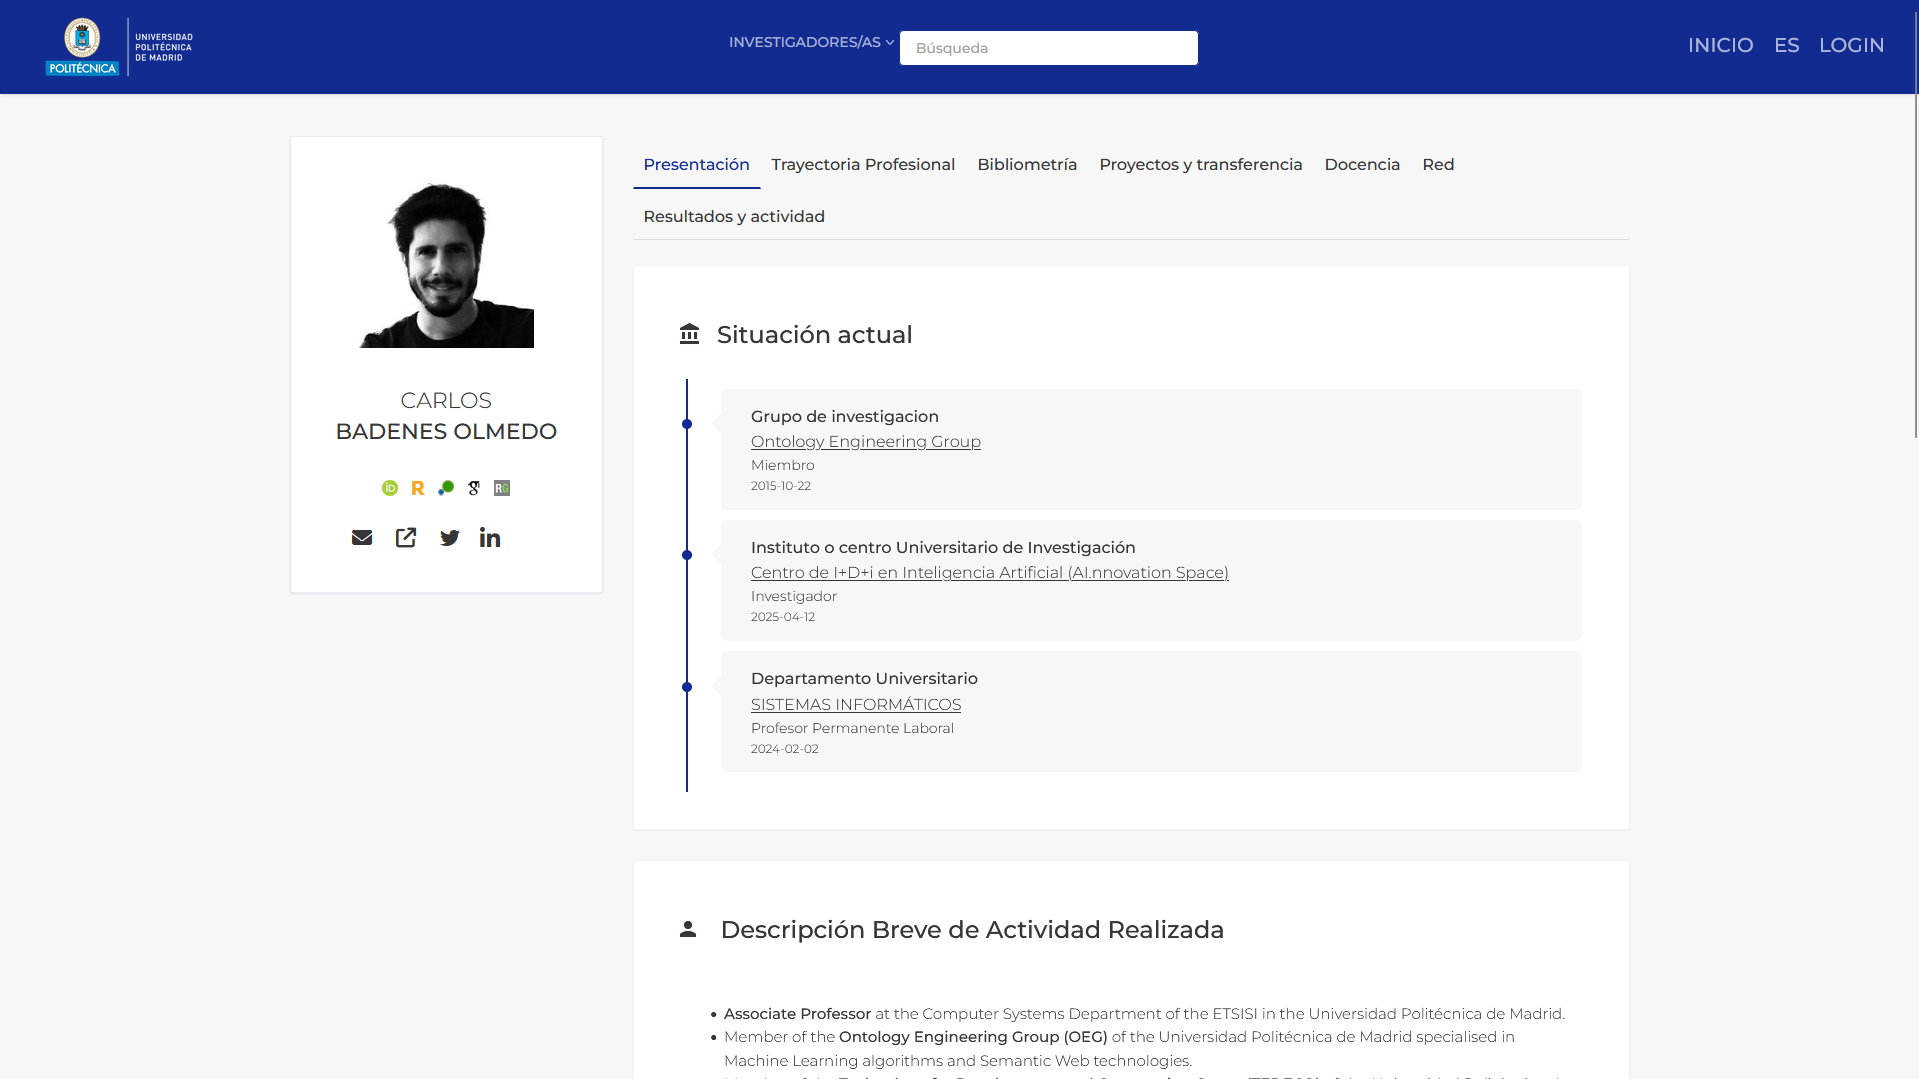
\includegraphics[width=\linewidth]{figures/portal_cientifico_1.png}
    \caption{Página inicial de un \gls{pdi} del Portal Científico.}
    \label{fig:portal-1}
  \end{subfigure}
  \hfill
  \begin{subfigure}{0.48\textwidth}
    \centering
    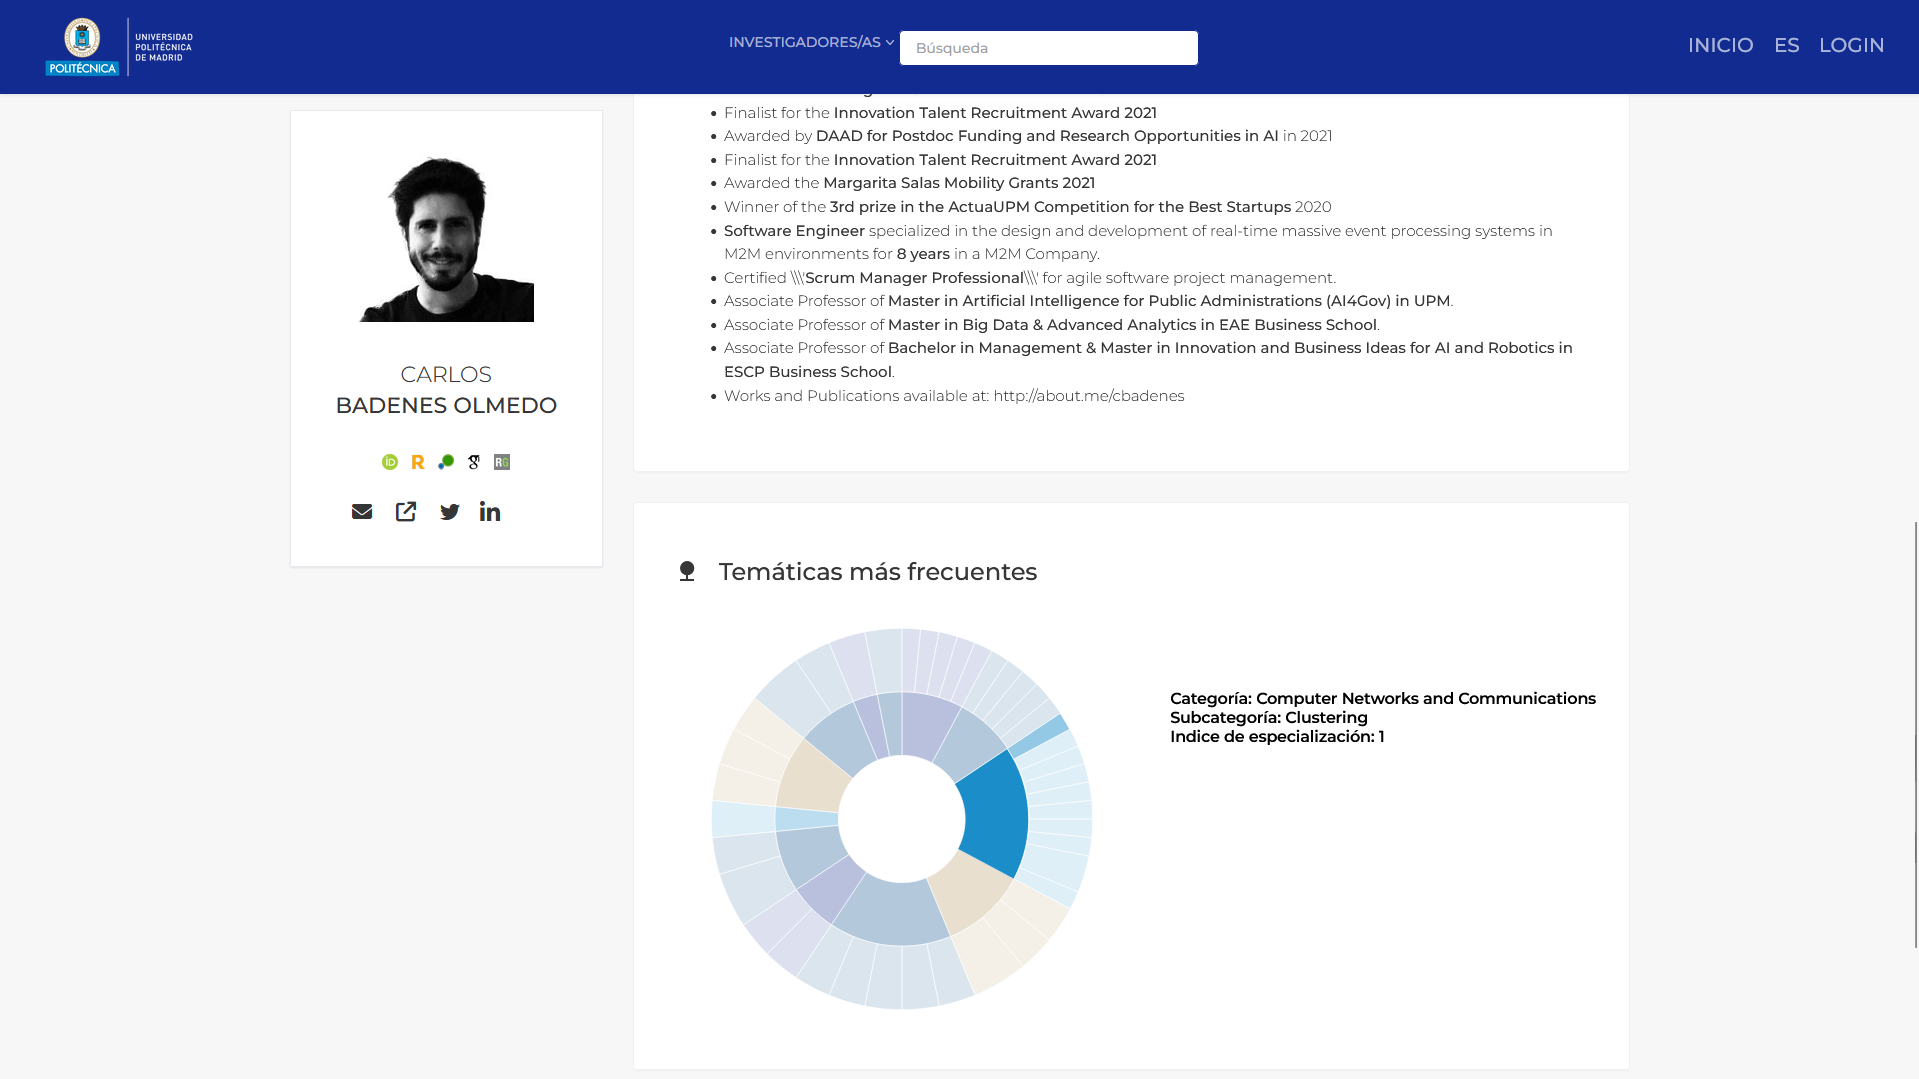
\includegraphics[width=\linewidth]{figures/portal_cientifico_2.png}
    \caption{Gráfico con los temas del \gls{pdi}.}
    \label{fig:portal-2}
  \end{subfigure}

  \vspace{4mm}

  \begin{subfigure}{\textwidth}
    \centering
    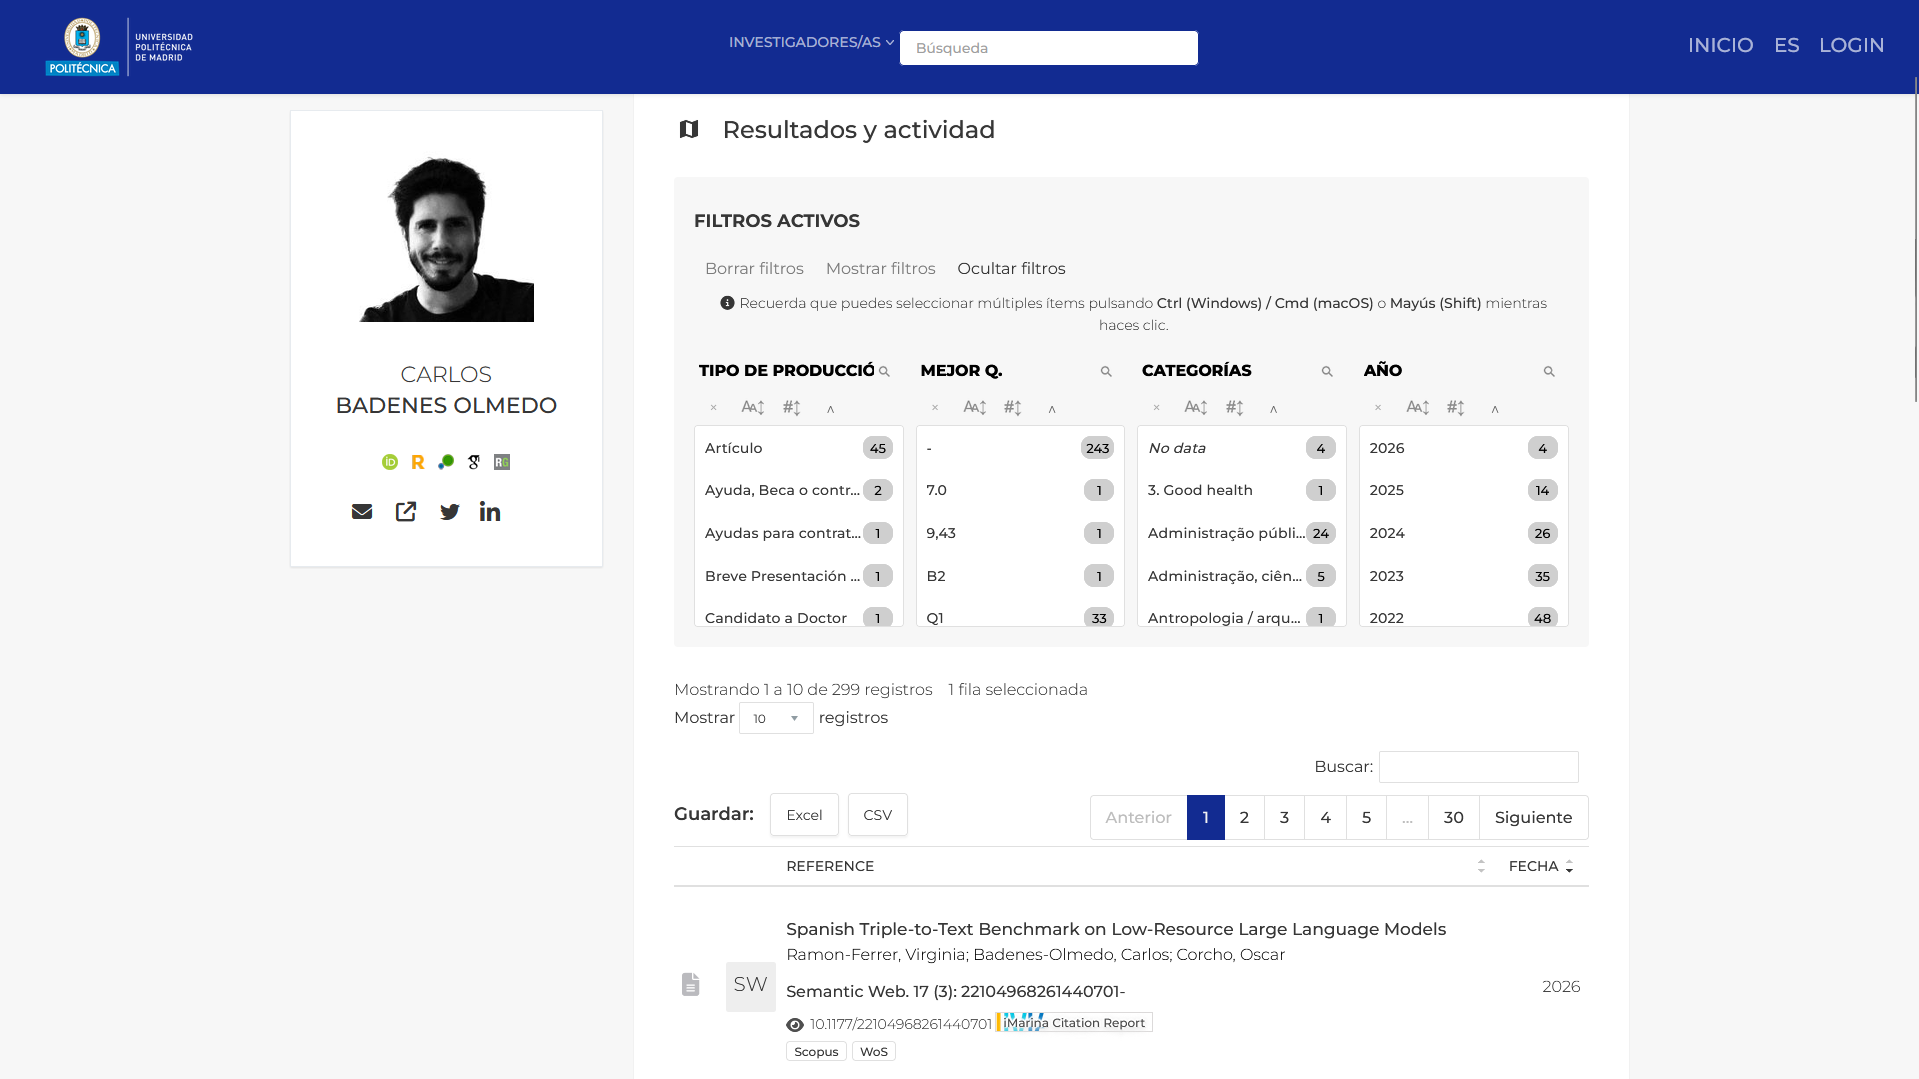
\includegraphics[width=0.90\linewidth]{figures/portal_cientifico_3.png}
    \caption{Sección de Resultados y actividad del \gls{pdi} con toda su información.}
    \label{fig:portal-3}
  \end{subfigure}

  \caption{Perfil público de un investigador en el Portal Científico de la \gls{upm}, tal como lo consulta hoy un estudiante: rico y bien presentado para la lectura humana ficha a ficha, pero no pensado para la exploración ni la comparación a escala.}
  \label{fig:portal}
\end{figure}

\pendiente{Mirar si tengo que anonimizar los datos de la captura}

Convertir esa fuente en un activo operativo exige, por tanto, un esfuerzo previo considerable: descubrir el censo de investigadores, descargar de forma respetuosa y reproducible las miles de páginas y transformar un marcado pensado para presentación visual en datos estructurados.
Es un trabajo de ingeniería poco vistoso, pero es la condición de posibilidad de todo lo demás.
Su ausencia explica que muchos intentos similares no pasen de la idea.
Esta barrera motiva el requisito~\ref{req:adquisicion} y se aborda en el objetivo~\ref{obj:adquisicion}.

\section{Heterogeneidad y ruido}
\label{sec:problema-heterogeneidad}

Aún una vez estructurados, los datos distan de ser homogéneos.
La densidad de los perfiles varía en órdenes de magnitud: conviven investigadores con cientos de publicaciones y décadas de actividad con perfiles prácticamente vacíos.
La Figura~\ref{fig:densidad} lo cuantifica sobre el perímetro: de los 995 investigadores, 219 (el 22\%) no tienen ninguna publicación registrada, mientras que 147 (casi el 15\%) superan el centenar y el más prolífico acumula 726.
La mediana, 17 publicaciones por investigador, queda muy por debajo de la media (46), reflejo de una distribución fuertemente sesgada.

\begin{figure}[htbp]
  \centering
  \begin{tikzpicture}
    \begin{axis}[
      upmhbar, height=5.2cm, xmax=255, bar width=12pt,
      symbolic y coords={c0,c1,c2,c3,c4,c5},
      ytick={c0,c1,c2,c3,c4,c5},
      yticklabels={0, 1--5, 6--20, 21--50, 51--100, {$>$100}},
      xlabel={Investigadores del perímetro},
      ylabel={Publicaciones por investigador},
      nodes near coords, nodes near coords style={font=\footnotesize\color{black!70}},
      clip=false,
    ]
      \addplot[fill=upmblue, draw=upmblue!60!black] coordinates {(219,c0)(135,c1)(176,c2)(184,c3)(134,c4)(147,c5)};
    \end{axis}
  \end{tikzpicture}
  \caption{Distribución del número de publicaciones por investigador en el perímetro (995 \glspl{pdi}). Los extremos conviven: 219 perfiles sin publicaciones registradas y 147 con más de cien (hasta un máximo de 726), lo que ilustra la heterogeneidad que la representación debe tolerar.}
  \label{fig:densidad}
\end{figure}

Los temas de investigación se expresan en vocabularios no controlados, con duplicados, variantes morfológicas y mezcla de idiomas.
Los resúmenes de las publicaciones presentan formatos idiosincrásicos que requieren una limpieza cuidadosa para no introducir ruido en las representaciones semánticas posteriores.

Esta heterogeneidad tiene una consecuencia metodológica clara: la representación de cada investigador debe tolerar perfiles incompletos y agregar toda la evidencia disponible (publicaciones, proyectos, temas declarados) en lugar de depender de un único campo bien cumplimentado.
Esta barrera motiva el requisito~\ref{req:normalizacion} y se aborda en los objetivos~\ref{obj:adquisicion} y~\ref{obj:perfilado}.

\section{La brecha de vocabulario entre estudiante e investigador}
\label{sec:problema-vocabulario}

La dificultad principal del emparejamiento es lingüística.
Un estudiante describe su interés en lenguaje coloquial, habitualmente en español y orientado a la aplicación («me gustaría detectar bulos en redes sociales»).
La actividad de un investigador, en cambio, queda registrada en el lenguaje de las publicaciones: técnico, mayoritariamente en inglés y orientado al método (\emph{misinformation detection}, \emph{transformer-based fact verification}).
Entre ambos registros media una doble brecha (tanto de idioma como de vocabulario) que hace fracasar la coincidencia léxica directa: los términos del estudiante, literalmente, no aparecen en el perfil del tutor idóneo.

Este fenómeno, identificado desde los orígenes de la recuperación de información como el \emph{problema del vocabulario} \citep{furnas1987vocabulary} (la constatación empírica de que dos personas eligen el mismo término para referirse a un mismo objeto con una probabilidad inferior al 20\%), es aquí especialmente severo por su carácter multilingüe, lo que constituye la razón técnica por la que una solución ingenua basada en búsqueda de palabras clave resulta insuficiente\duda{No me gusta esta afirmación, no deberíamos poder afirmar esto tan pronto}.
Abordarlo exige representaciones que capturen proximidad semántica más allá de la superficie léxica, o mecanismos que traduzcan y expandan la consulta del estudiante hacia el registro de los perfiles, idealmente, ambas cosas (se abordan en el Capítulo~\ref{ch:sota}).
Esta barrera motiva el requisito~\ref{req:emparejamiento} y se aborda en los objetivos~\ref{obj:perfilado} y~\ref{obj:emparejamiento}.

\section{La ausencia de verdad de referencia}
\label{sec:problema-groundtruth}

Supongamos construido el sistema: ¿cómo saber si recomienda bien? Evaluar un recomendador de tutores requiere pares (consulta, tutor correcto), y obtenerlos por etiquetado manual es costoso y delicado: exigiría que expertos conocedores de toda la plantilla juzgaran, para cada consulta, qué investigadores son pertinentes, convirtiendo el problema en un juicio subjetivo, caro y difícilmente reproducible.

Esta carencia de verdad de referencia es, a nuestro juicio,\duda{Puedo poner valoraciones personales?} una de las razones de fondo por las que las herramientas de este tipo rara vez superan la fase de demostración: sin evaluación objetiva no hay forma de comparar alternativas ni de justificar mejoras y el desarrollo se estanca en la anécdota.
Este trabajo propone una salida: explotar la \emph{historia real de supervisión} (los trabajos que cada investigador ha dirigido efectivamente) como fuente automática de \emph{pares consulta-respuesta} (Capítulo~\ref{ch:evaluacion}).
Esta barrera motiva el requisito~\ref{req:evaluacion} y se aborda en el objetivo~\ref{obj:evaluacion}.

\section{Restricciones institucionales: soberanía del dato y coste}
\label{sec:problema-institucional}

Por último, el contexto de despliegue impone restricciones propias.
Una herramienta institucional que procesa consultas de estudiantes y perfiles de empleados públicos no debería depender de servicios de inteligencia artificial de terceros: el envío sistemático de esos datos a APIs externas plantea reservas de gobernanza y genera un coste recurrente difícil de asumir y de justificar.
A ello se suma la exigencia práctica de que el sistema completo sea operable por la propia institución con recursos modestos.

Hasta hace muy poco, esta restricción era casi eliminatoria: la calidad necesaria para interpretar consultas y sintetizar perfiles solo la ofrecían modelos propietarios accesibles por \gls{api}.
La reciente madurez de los modelos de lenguaje abiertos ejecutables en local (y de los ecosistemas para servirlos) cambia ese panorama y abre, por primera vez, la posibilidad de un sistema de esta naturaleza íntegramente \emph{on-premise}.
Este trabajo adopta esa vía y la somete a prueba.
Esta barrera motiva el requisito~\ref{req:soberania} y se aborda en el objetivo~\ref{obj:prototipo}.

\section{Síntesis: requisitos de la solución}
\label{sec:problema-requisitos}

Del análisis anterior se desprende que el problema sigue abierto no por falta de técnicas, sino porque su resolución exige atravesar \emph{todas} las barreras a la vez: sin adquisición no hay datos, sin normalización no hay perfiles, sin representación semántica no hay emparejamiento útil, sin verdad de referencia no hay progreso medible y sin despliegue local no hay adopción institucional.
La Tabla~\ref{tab:requisitos} resume esta correspondencia entre problemas y requisitos, que actúa como hilo conductor del resto de la memoria.

\begin{table}[htbp]
    \centering
    \caption{Correspondencia entre las barreras identificadas, los requisitos de diseño del sistema y los objetivos que los abordan.}
    \label{tab:requisitos}
    \begin{tabularx}{\textwidth}{l X X c}
        \toprule
        \rowcolor{upmblue!8} \colhead{Id.} & \colhead{Barrera} & \colhead{Requisito derivado} & \colhead{Objetivo} \\
        \midrule
        \reqid{req:adquisicion} & Fuente pública no operativa (\ref{sec:problema-datos}) & Adquisición automatizada, incremental y reproducible de los datos del portal. & \ref{obj:adquisicion}\\
        \reqid{req:normalizacion} & Heterogeneidad y ruido (\ref{sec:problema-heterogeneidad}) & Perfiles normalizados que agreguen toda la evidencia disponible y toleren datos incompletos. & \ref{obj:adquisicion}, \ref{obj:perfilado}\\
        \reqid{req:emparejamiento} & Brecha de vocabulario e idioma (\ref{sec:problema-vocabulario}) & Emparejamiento robusto al desajuste léxico y translingüe entre consulta y perfil. & \ref{obj:perfilado}, \ref{obj:emparejamiento}\\
        \reqid{req:evaluacion} & Ausencia de verdad de referencia (\ref{sec:problema-groundtruth}) & Evaluación objetiva y reproducible sin etiquetado manual. & \ref{obj:evaluacion}\\
        \reqid{req:soberania} & Soberanía del dato y coste (\ref{sec:problema-institucional}) & Despliegue íntegro en infraestructura propia, con modelos abiertos y coste marginal nulo por consulta. & \ref{obj:prototipo}\\
        \bottomrule
    \end{tabularx}
\end{table}